\subsection{Problem Formulation}

\emph{Problem-solving} agents are able to search for a sequence of actions that result in a solution to a problem, which can then be applied to the problem to solve it.
This is known as the \emph{search~approach}.
An algorithm that searches for a solution to a \emph{search problem} is a \emph{search algorithm}.
An \emph{uninformed} search algorithm is given no information regarding states, other than the \emph{problem formulation}.

The elements of a problem formulation are
\begin{itemize}
  \item the initial state,
  \item the goal states,
  \item possible actions and their effects on states, and
  \item a cost function.
\end{itemize}

A goal state is a desired outcome of the problem.
A solution is a sequence of actions that lead from the initial state to a goal state.
The best solution is that with the lowest cost.
Typically, the cost of a solution is the sum of the costs of its actions.

A \emph{state~space graph} contains all the possible states of the problem.
It is implicitly defined by the initial state, and the possible actions and their effects on states.
A solution is a path through the state~space graph.
Some solutions are better than others.
It is not necessary to give the state~space graph as an input to a search algorithm.
Only the problem formulation is necessary.

\subsection{Search Trees}

A search tree is generated by a search algorithm in order to search for a solution.
Each node in the tree represents a state of the problem.
The root node represents the initial state of the problem.
Each connection between a pair of nodes corresponds to an action that transforms the state of the first node to the state of the second node.

In order to save memory, a search tree represents only the explored portion of the graph.
When a node has been expanded, it is often circled on the search tree diagram.
An expanded node is said to have been \emph{visited}.
The set of nodes in the tree that are available to be expanded is known as the \emph{frontier}.

Different search algorithms correspond to different ways of deciding which frontier node to visit next.
Breadth-first and depth-first searches are techniques that can be used when the costs of each action are the same.

\subsection{Breadth-First Search}

To perform a \emph{breadth-first} search
\begin{enumerate}
  \item visit the shallowest frontier node first, placing its children in the frontier, but
  \item do not place a child in the frontier if its corresponding state is represented by a node already in the frontier or the list of visited nodes.
  \item Stop searching when a goal node is placed in the frontier.
\end{enumerate}

Breadth-first search can be seen as a first-in, first-out (FIFO) algorithm.
The frontier is a FIFO queue, in which the earliest node is the first to be visited.

The search finds a solution for a given problem formulation.
The cost of the search is expressed in terms of its time and space complexity.
The cost of a solution is typically the sum of the costs of its actions.

A breadth-first search with a branch factor \( b \) (maximum number of children per node) and a shallowest goal depth \( d \) (where the root has a depth of zero) has the following properties.
\begin{itemize}
  \item It is complete --- as long as \( b \) is finite, the search is guaranteed to find a path to a goal state if one exists, or to terminate in failure otherwise.
  \item It is optimal --- the search is guaranteed to find the shortest path to a goal state, as long as all actions have the same cost.
  \item It has a worst-case space complexity of \( \function{O}{b^{d}} \).
  \item It has a worst-case time complexity of \( \function{O}{b^{d}} \).
\end{itemize}

The complexity \( \function{O}{b^{d}} \) means that in the worst case, the algorithm must generate and store \( b^{d} \) nodes, which may require a large amount of time and memory.
Thus, breadth-first search is not an efficient algorithm, and is not recommended for large problems.

\subsection{Depth-First Search}

To perform a \emph{depth-first} search
\begin{enumerate}
  \item visit the deepest frontier node first, placing its children in the frontier, but
  \item do not place a child in the frontier if its corresponding state is represented by a node already in the frontier or the list of visited nodes.
  \item Stop searching when a goal node is visited.
\end{enumerate}

Unlike a breadth-first search, a depth-first search does not stop until a goal node is visited, or all nodes are visited without reaching a goal node.
The rationale is to visit or expand every node in a branch until it cannot be expanded any further, or a goal node is found, before moving to another branch.

Depth-first search can be seen as a last-in, first-out (LIFO) algorithm.
The frontier is a LIFO stack, in which the latest node is the first to be visited.

A depth-first search has the following properties.
\begin{itemize}
  \item It is complete if the state space is finite --- if the state space is finite, the search is guaranteed to find a path to a goal state if one exists, or to terminate in failure otherwise
  \item It is not complete if the state space is infinite.
  \item It is not optimal --- it is not guaranteed to find the shortest path to a goal state.
  \item It has a worst-case space complexity of the order of the size of the state space.
  \item It has a worst-case time complexity of the order of the size of the state space.
\end{itemize}

A complexity of the order of the size of the state space means that in the worst case, the algorithm must generate and store the entire state space graph.

\subsection{Space-Saving Depth-First Search}

The standard depth-first search stores all previously visited states to ensure that the algorithm is complete when the state space is finite.
If previously visited states were not stored, it is possible that states may eventually be revisited, which may cause an infinite loop.

Memory could be saved without affecting completeness by only storing the nodes (and their unvisited siblings) in the path from the root to the current node.
For a search tree with a maximum depth of \( m \), this would have the following properties.
\begin{itemize}
  \item It has a reduced worst-case space complexity of \( \function{O}{b m} \).
  \item It has a reduced worst-case time complexity of \( \function{O}{b^{m}} \).
\end{itemize}

\subsection{Space-Saving Depth-Limited Search}

In order to guarantee that a depth-first search will terminate in a reasonable amount of time, a limit can be placed on the maximum search depth.
A \emph{depth-limited} search is a depth-first search to a maximum depth of \( L \), where the root node has a depth of zero.

To perform a depth-limited search
\begin{enumerate}
  \item visit the deepest frontier node first, placing its children in the frontier only if the depth \( d \) of the children is less than or equal to the depth limit \( L \), but
  \item do not place a child in the frontier if its corresponding state is represented by a node already in the stored frontier or the list of visited nodes.
  \item Stop searching when a goal node is visited.
\end{enumerate}

A space-saving depth-limited search with its shallowest goal at depth \( d \) has the following properties.
\begin{itemize}
  \item It is complete if \( d \leq L \).
  \item It is not optimal --- like the standard depth-first search, it is not guaranteed to find the shortest path to a goal state.
  \item It has a reduced worst-case space complexity of \( \function{O}{b L} \).
  \item It has a reduced worst-case time complexity of \( \function{O}{b^{L}} \).
\end{itemize}

Thus, the depth-limited search has the same or greater time complexity as a breadth-first search.

\begin{figure}[htp]
  \centering
  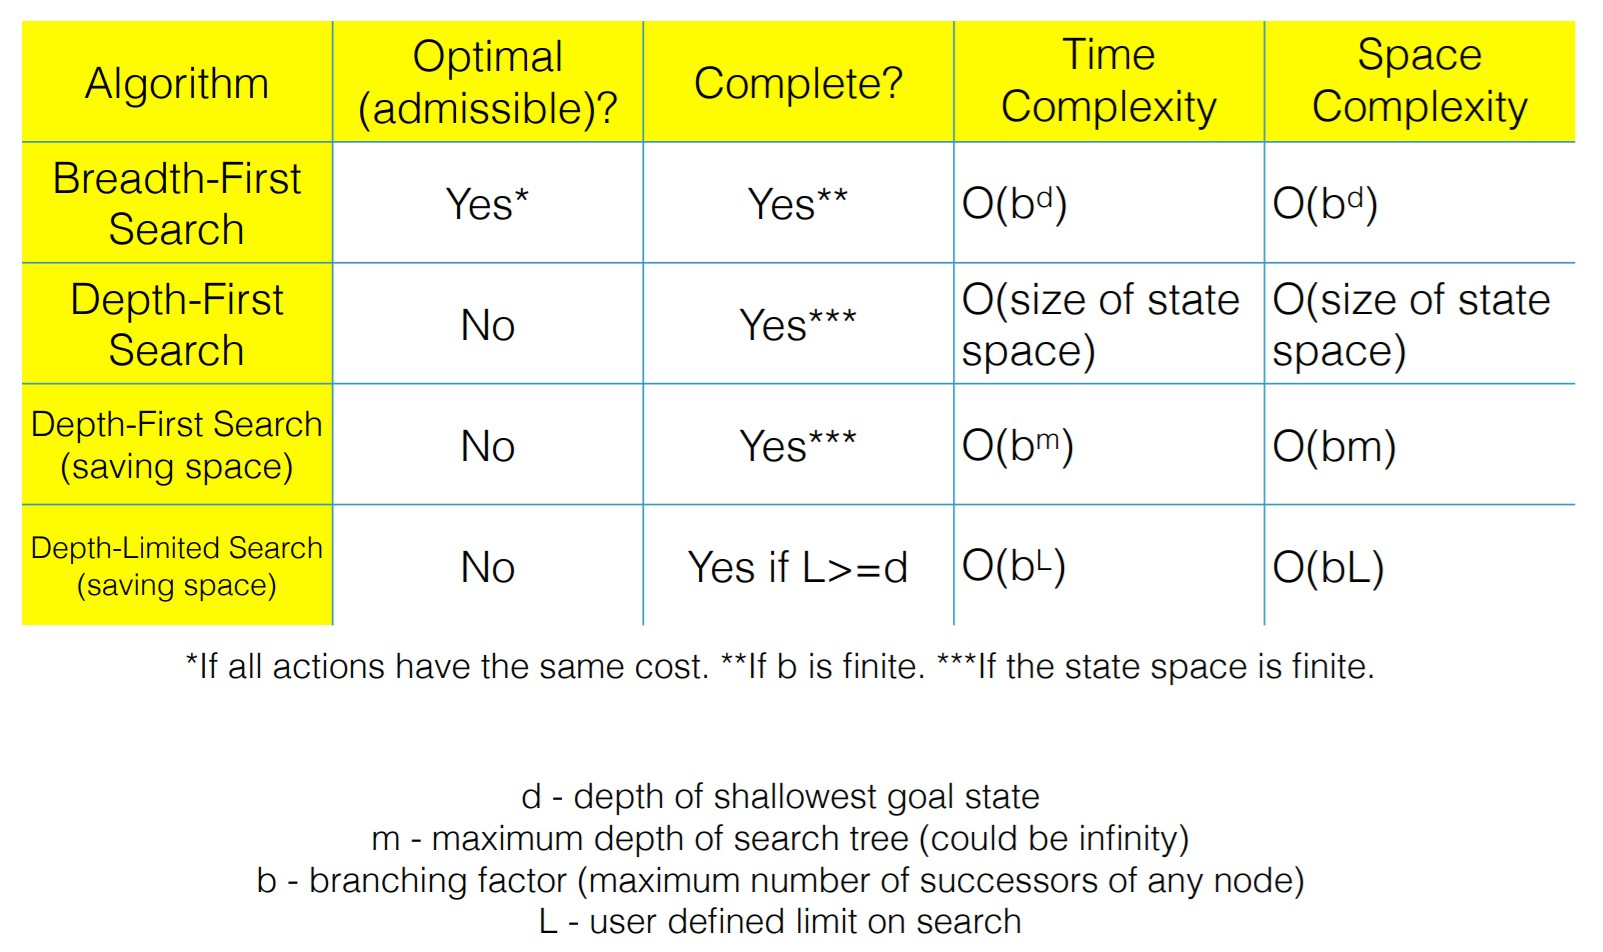
\includegraphics[width=0.8\textwidth]{unit-8/figures/uninformed-search-comparison.jpg}
  \caption*{Comparison of uninformed search algorithms.}
\end{figure}
